\documentclass[bsc]{report/media/abdnthesis}

\usepackage{report/00-preamble}

\title{Integrating Differential Privacy into Fluent Bit}
\author{Julien Leo Acker}

\school{Department of Computing Science}
    
\date{2024}

\begin{document}

\maketitle
\makedeclaration

\begin{abstract}
This project aims to develop a Filter plugin for Fluent Bit that implements additive noise \acrlong{dp} techniques to protect individual privacy while allowing for valuable insights to be derived from sensitive data. Differential Privacy has emerged as a leading standard for privacy-preserving data analysis, providing a rigorous framework to quantify and control the privacy loss incurred when performing statistical analyses on sensitive data. However, many existing DP implementations lack the portability needed for widespread adoption.

To address this challenge, the project presents a Rust-based filter plugin that is compiled to a WebAssembly (WASM) target, which Fluent Bit, an industry-standard open-source log and metric processor, loads and executes in a sandboxed environment. The plugin applies the Laplacian mechanism for $\epsilon$-differential privacy and the Gaussian mechanism for $(\epsilon, \delta)$-differential privacy. By adding carefully calibrated noise to the data based on the sensitivity of the function and the privacy budget $\epsilon$, the plugin ensures that the presence or absence of any individual's data does not significantly affect the analysis results.

The WASM-based architecture enables the DP algorithms to run seamlessly across different platforms, taking advantage of Fluent Bit's high-performance data processing capabilities. The plugin's settings for each data stream are loaded from TOML configuration files, allowing for flexible and dynamic control over the privacy parameters. Evaluation of the plugin's effectiveness and performance is conducted using sample datasets and a Jupyter Notebook to analyze the utility and privacy of the perturbed data.

This project demonstrates the feasibility of integrating DP into a production-ready log processing framework using WASM for enhanced portability and security. It provides a solid foundation for privacy-preserving data analysis within Fluent Bit's extensible plugin ecosystem, enabling the protection of sensitive information while still allowing for valuable insights to be gained from the data. The project's outcomes contribute to the broader goal of making privacy-preserving techniques more accessible and easier to deploy in real-world scenarios.

Future work could focus on expanding the range of supported probability distributions and DP algorithms, as well as exploring the integration of the plugin with other data processing frameworks. By building upon this project's findings and extending its capabilities, researchers and practitioners can continue to advance the field of privacy-preserving data analysis and work towards a more secure and trustworthy data ecosystem.
\end{abstract}

\begin{acknowledgements}
I would like to thank Chunyan Mu for supervising me for this project. Giving helpful advice and ensuring that I stay on track with the assignment.

I would like to acknowledge that Fluent Bit's Documentation around WASM support is reasonably exhaustive. I loosely based my filter plugin on the example Rust WASM plugin they host in their main repository. I very loosely adapted parts of their Dockerfile when writing the Fluent Bit build-stage in my own Dockerfile.

\end{acknowledgements}

\def\sfthing#1#2{\def#1{\mbox{{\small\normalfont\sffamily #2}}}}

\sfthing{\PP}{P}
\sfthing{\FF}{F}

\printglossary[type=\acronymtype]
\printglossary
\tableofcontents
\listoftables
\listoffigures
\lstlistoflistings{}

\chapter{Introduction\label{chap:introduction}}
\section{Overview}

This project focuses on the development of a Rust-based Filter plugin for Fluent Bit that integrates Differential Privacy techniques to protect the privacy of individuals in data streams while allowing for valuable insights to be derived from the data. The filter plugin applies Differential Privacy by adding noise drawn from either a Laplace or Gaussian distribution to numeric data based on user-defined settings. The plugin is compiled to a WebAssembly (WASM) binary, which Fluent Bit loads and executes in a sandboxed environment, ensuring portability and security.

To evaluate the effectiveness and performance of the filter plugin, an evaluation infrastructure is created using a multi-stage Dockerfile. The infrastructure compiles the filter plugin to WASM, builds Fluent Bit with WASM support, and optionally pre-optimizes the WASM binary using Ahead-of-Time (AOT) compilation for improved performance. The filter plugin is then executed by Fluent Bit, processing two sample datasets according to a provided configuration file. The results are saved to output files and loaded into a Jupyter Notebook for analysis and visualization.

\section{Research Question}
The central research question addressed by this project is:
\textit{How can Differential Privacy be effectively integrated into a high-performance data processing pipeline, such as Fluent Bit, to protect individual privacy while maintaining data utility and ensuring portability across various environments?}
By answering this question, the project aims to contribute to the field of privacy-preserving data analysis and provide a practical solution for applying Differential Privacy in real-world scenarios.
\section{Objectives}
The main objectives of this project are:
\begin{enumerate}
\item Develop a Rust-based Filter plugin for Fluent Bit that applies Differential Privacy techniques to numeric data using the Laplace and Gaussian mechanisms.
\item Compile the filter plugin to a WASM target to ensure compatibility with Fluent Bit's WASM plugin system and enable portability across different platforms.
\item Design a flexible configuration system using TOML files to allow users to specify privacy settings for each data stream.
\item Integrate the WASM plugin into Fluent Bit, ensuring proper data flow and error handling.
\item Create an evaluation infrastructure using Docker to demonstrate the plugin's functionality and performance on sample datasets.
\item Analyze the results using a Jupyter Notebook to assess the impact of Differential Privacy on data utility and privacy.
\end{enumerate}
\section{Contributions}
The primary contributions of this project are:
\begin{itemize}
\item A novel implementation of Differential Privacy techniques in a WASM-based filter plugin for Fluent Bit, enabling privacy-preserving data processing in a high-performance, portable, and secure manner.
\item A flexible configuration system that allows users to easily specify and adjust privacy settings for each data stream, facilitating the adoption of Differential Privacy in various scenarios.
\item An evaluation infrastructure that demonstrates the effectiveness and performance of the filter plugin on sample datasets, providing insights into the impact of Differential Privacy on data utility and privacy.
\item A comprehensive analysis of the results, highlighting the trade-offs between privacy and utility and offering guidance for applying Differential Privacy in real-world data processing pipelines.
\end{itemize}
By addressing the challenges of integrating Differential Privacy into a widely-used open-source log processor like Fluent Bit, this project contributes to the broader goal of making privacy-preserving data analysis more accessible and easier to deploy across various environments. The project's outcomes have the potential to facilitate the adoption of Differential Privacy in a wide range of applications, ultimately leading to better protection of individual privacy while still enabling valuable insights to be derived from sensitive data.

\section{Motivation}
The increasing collection and analysis of personal data have led to growing concerns about privacy and the potential misuse of sensitive information. Differential Privacy has emerged as a strong standard for privacy-preserving data analysis, providing rigorous guarantees while still allowing for accurate statistical insights. However, integrating Differential Privacy into real-world data processing pipelines can be challenging due to the lack of portable, high-performance implementations that can be easily deployed across various platforms and languages.

Fluent Bit, a lightweight and highly efficient log processor and forwarder, presents an ideal opportunity to address this challenge. By creating a WASM-based Differential Privacy plugin for Fluent Bit, this project aims to make privacy-preserving data analysis more accessible and easier to integrate into existing data processing workflows. The use of WASM ensures portability across different environments, while Fluent Bit's high-performance architecture enables the application of Differential Privacy techniques without significant overhead.

Moreover, by integrating Differential Privacy at the data ingestion and processing stage, this project allows for the protection of sensitive information early in the data pipeline, reducing the risk of privacy breaches and ensuring that data is anonymized before being stored or analyzed further downstream. This approach promotes a proactive stance towards privacy, aligning with the principles of privacy by design.

The motivation behind this project lies in the belief that privacy should be a fundamental right and that technological solutions, such as Differential Privacy, can play a crucial role in safeguarding individual privacy while still enabling the benefits of data-driven decision-making. By making Differential Privacy more accessible and easier to implement through the development of a WASM-based plugin for Fluent Bit, this project seeks to contribute to the wider adoption of privacy-preserving techniques in real-world scenarios, ultimately leading to a more secure and trustworthy data ecosystem.
\chapter{Background \& Related Work\label{chap:background}}

\section{Differential Privacy}

\acrfull{dp} is a mathematical framework for protecting individual privacy in datasets while allowing statistical analysis and insights to be derived from the data \cite{Dwork2006calibrating,Dwork2014}. It involves adding controlled noise to individual records to preserve privacy without diminishing utility beyond desired bounds \cite{WhatisDifferentialPrivacy}. Striking the correct balance between privacy and utility is at the heart of \acrshort{dp} research \cite{Dwork2014}. \acrshort{dp} aids in regulatory compliance and is widely deployed, often using bespoke implementations, to anonymize telemetry data on iOS, Android, Windows, and Chrome \cite{Maranon,markdefalco_2020}. Active research is conducted by both academia and industry, with notable groups including Microsoft's AI Lab, Google Research, Harvard's Privacy Tools Project, and Apple's Machine Learning Research - Differential Privacy Team.

\subsection{Foundations and Key Concepts}

The seminal work by \citet{Dwork2006calibrating} introduced \acrshort{dp}, proposing a mechanism for privacy-preserving statistical database queries by adding calibrated noise to query outputs. This work showed that privacy could be preserved by adjusting the noise scale according to the sensitivity of the computed function, ensuring that the presence or absence of any individual in the dataset does not significantly affect the analysis outcome. Subsequent research explored \acrshort{dp} mechanics, focusing on mechanisms that add noise to query outputs based on sensitivity \cite{Dwork2006calibrating}. The Laplace mechanism was introduced for adding scaled noise to ensure individual data does not significantly affect query outputs. The Gaussian mechanism was proposed as an alternative, offering better privacy-accuracy trade-offs under certain conditions \cite{Dwork2014}.
Additional concepts, such as privacy budget \cite{McSherry2007} and composability of \acrshort{dp} \cite{Dwork2014}, were introduced to highlight the cumulative nature of privacy loss across multiple queries and the importance of managing the budget to maintain robust guarantees. The distinction between global and local \acrshort{dp} was also made, differentiating between privacy guarantees provided by a trusted curator versus those provided in a decentralized manner \cite{kasiviswanathan2010learn}.

\subsection{Challenges and Open Problems}
Despite its emergence as a strong standard for privacy-preserving data analysis, \acrshort{dp} still faces challenges in practical implementation and adoption. The primary issue is the trade-off between privacy and utility, as adding noise to protect privacy can degrade the accuracy and usefulness of analysis results \cite{Dwork2014}. Balancing these competing objectives requires careful tuning of privacy parameters. Composition of \acrshort{dp} guarantees across multiple queries or analyses is another challenge, as each query consumes a portion of the privacy budget, and cumulative privacy loss must be tracked and controlled \cite{mcsherry2007mechanism}. Choosing appropriate sensitivity and privacy budget parameters is also crucial, as these values directly impact the privacy-utility trade-off \cite{Dwork2006calibrating}. Furthermore, implementing \acrshort{dp} mechanisms can be non-trivial, requiring careful attention to numerical stability, randomness generation, and code correctness to ensure the implementation accurately reflects the theoretical guarantees \cite{Mironov2012}.

\section{Existing Implementations of Differential Privacy}
Several software implementations aim to make \acrshort{dp} more practical and accessible to data analysts and scientists. This section reviews some of the most notable implementations.

\subsection{Google's Differential Privacy Library}
Google's commitment to \acrshort{dp} has evolved significantly since its early RAPPOR project in 2014. In 2019, Google launched an open-source \acrshort{dp} library written in C++, allowing developers to implement \acrshort{dp} in their applications \cite{Guevara_2022,RAPPOR,wilson2019differentially}. The library provides tools and features to facilitate \acrshort{dp} implementation, including mechanisms, algorithms, statistical functions, testing frameworks, and modular components \cite{wilson2019differentially,wilson2020differentially,RAPPOR}. It supports various programming languages and has been utilized in Google products like Maps and BigQuery \cite{Google_BigQuery}.

\subsection{Apple's Differential Privacy}
Apple has been a pioneer in deploying \acrshort{dp} at scale, first announcing its use in 2016 for collecting user data to improve services \cite{tang2017privacy,AppleDifferentialPrivacy2017}. Apple's implementation relies on a local model, adding noise to data on the user's device before sending it to servers, ensuring Apple only learns aggregate statistics. The technology is built into the core of Apple's operating systems and is used for various purposes, with technical whitepapers detailing the implementation and privacy guarantees \cite{AppleDifferentialPrivacy2017}.

\subsection{Microsoft's Differential Privacy Implementation}
Microsoft has contributed to \acrshort{dp} through theoretical research and practical implementations. A notable contribution is the SmartNoise system, developed in collaboration with Harvard as part of the OpenDP initiative \cite{MicrosoftOpenDP,MicrosoftHarvardOpenDP}. SmartNoise enables researchers and data scientists to derive insights from datasets while preserving individual privacy by adding statistical noise and managing a privacy-loss budget \cite{MicrosoftDataResponsibly}. Microsoft has applied \acrshort{dp} to Windows telemetry data and LinkedIn advertiser queries \cite{MicrosoftDataResponsibly}. While not directly applicable to the Fluent Bit filter plugin, Microsoft's work demonstrates the feasibility of deploying \acrshort{dp} in production environments.


\subsection{OpenDP}
OpenDP is a community effort to build an open-source suite of tools for deploying differential privacy \cite{opendp2020, Vadhan2019OpenDPA}. It consists of several projects and libraries in multiple languages, including a Rust-based library developed by researchers from Harvard that implements many common \acrshort{dp} algorithms. This was the initially planned library to provide the distributions for the Filter plugin implementation. However due to technical issues, it was found significantly simpler to use the \texttt{Rv} Rust crate due to it's more focused nature. More details can be found in the relevant design and implementation sections.

\subsection{Other Notable Implementations}
The US Census Bureau has adopted \acrshort{dp} as the new standard for protecting individual privacy in its data releases, using the TopDown algorithm to add noise hierarchically \cite{Gong2022Harnessing}. IBM's Diffprivlib is an open-source Python library for experimenting with \acrshort{dp}, designed for ease of use and providing a simple API for applying \acrshort{dp} to data analysis tasks \cite{holohan2019diffprivlib}.


\section{Fluent Bit}
Fluent Bit is an industry-standard open source Log and Metric processor capable of taking in events from a large variety of sources, applying filters, buffering, and then sending the processed data to a variety of destinations.\cite{What-is-Fluent-Bit} Written in C, it's YAML-based configuration defines a graph structure for where events should be sourced, what to do with the event, and where the event should be eventually sent. For example: a hub device running Fluent Bit could take in logs from a connected IoT device via MQTT, it then can extract a metric contained in the string, create a histogram based on those stored values, buffer the values to a persistent disk, then send the stored data to a remote server over your desired protocol.
\subsection{Other WASM plugins}
An example of a plugin that leverages Fluent Bit's WASM filter plugin support is \textit{flb\_filter\_iis}\cite{Ortega}, which processes W3C's IIS-formatted logs into JSON to be consumed by Fluent Bit. It is an example of what's possible with stateless Rust WASM plugins for Fluent Bit, as it opens the door for using many Rust-native libraries in a containarized and portable environment. 
\chapter{Design\label{chap:design}}
\section{Differential Privacy Design}
Differential Privacy (DP) is a mathematical framework for protecting individual privacy in datasets while allowing statistical analysis. It achieves this by adding carefully calibrated noise to the data or query results. The amount of noise added depends on the \textit{sensitivity} of the query function (how much the output can change by modifying a single record) and the desired level of privacy, quantified by the \textit{privacy budget} $\epsilon$. 

This project implements two key mechanisms for achieving differential privacy: the Laplace Mechanism for $\epsilon$-DP and the Gaussian Mechanism for $(\epsilon, \delta)$-DP. The following subsections detail these mechanisms and their underlying probability distributions.

\subsection{Laplace Mechanism}
The Laplace Mechanism achieves $\epsilon$-differential privacy by adding noise drawn from the Laplace distribution to the output of a function $f$. The scale parameter $b$ of the distribution is set to $\Delta f / \epsilon$, where $\Delta f$ is the $L_1$ sensitivity of $f$, defined as the maximum change in $f$'s output that can result from modifying a single record.

\begin{definition}[Laplace Mechanism]
Given any function $f: \mathbb{N}^{|\mathcal{X}|} \rightarrow \mathbb{R}^k$, the Laplace Mechanism is defined as:
\begin{equation}
\mathcal{M}_L(x, f, \epsilon) = f(x) + (Y_1, \ldots, Y_k)
\end{equation}
where $Y_i$ are independent and identically distributed random variables drawn from $Lap(\Delta f/\epsilon)$, the Laplace distribution with scale $b = \Delta f/\epsilon$\citep[Def. 3.3]{Dwork2014}.
\end{definition}

The Laplace distribution has probability density function:
\begin{equation}
Lap(x | b) = \frac{1}{2b} \exp\left(-\frac{|x|}{b}\right) 
\end{equation}
Its mean is 0 and variance is $2b^2$\citep[Def. 3.2]{Dwork2014}. The Laplace Mechanism is implemented in this project using the \texttt{rv::dist::Laplace} distribution, with $\epsilon$ and sensitivity provided via configuration files.

\subsection{Gaussian Mechanism}
The Gaussian Mechanism relaxes $\epsilon$-DP to $(\epsilon,\delta)$-DP, where $\delta$ allows a small probability of violating strict $\epsilon$-DP. It adds Gaussian noise scaled to the $L_2$ sensitivity $\Delta_2 f$ and privacy parameters $\epsilon, \delta$.

\begin{definition}[Gaussian Mechanism]
Given any function $f: \mathbb{N}^{|\mathcal{X}|} \rightarrow \mathbb{R}^k$, the Gaussian Mechanism is defined as: 
\begin{equation}
\mathcal{M}_G(x, f, \epsilon, \delta) = f(x) + (Y_1, \ldots, Y_k)
\end{equation}
where $Y_i$ are independent and identically distributed random variables drawn from $\mathcal{N}(0, \sigma^2)$, the Gaussian distribution with mean 0 and variance $\sigma^2 = 2\ln(1.25/\delta)(\Delta_2 f)^2 / \epsilon^2$ \citep[Thm. 3.22]{Dwork2014}.
\end{definition}

The $L_2$ sensitivity $\Delta_2 f$ is the maximum $L_2$ distance between $f(x)$ and $f(y)$ for any two datasets $x, y$ differing in a single record. Intuitively, the noise variance $\sigma^2$ is proportional to $(\Delta_2 f)^2$ (more sensitive functions require more noise) and inversely proportional to $\epsilon^2$ (stricter privacy requires more noise). The term $2\ln(1.25/\delta)$ allows a $\delta$ probability of breaching $\epsilon$-DP.

The Gaussian Mechanism is implemented using \texttt{rv::Gaussian} with mean 0 and standard deviation calculated from the provided $\epsilon$, $\delta$, and $L_2$ sensitivity values.

\subsection{Sensitivity Calculation}
Both mechanisms require calculating the sensitivity of the query function. For the count, sum, and average queries supported in this project, the $L_1$ and $L_2$ sensitivities are straightforward:
\begin{itemize}
    \item \textbf{Count:} $\Delta f = \Delta_2 f = 1$, since adding or removing one record changes the count by at most 1.
    \item \textbf{Sum:} For a dataset with values in $[0, m]$, $\Delta f = m$ and $\Delta_2 f = m$ since a single record can change the sum by up to the maximum value $m$.
    \item \textbf{Average:} For a dataset with $n$ records and values in $[0,m]$, $\Delta f = m/n$ and $\Delta_2 f = m/n$ by the triangle inequality, since changing one record by $m$ changes the sum by $m$ and the average by $m/n$.
\end{itemize}
The project currently requires the user to manually specify the sensitivity values in the configuration files. Future work could involve automatically deriving sensitivities from the data schema and value ranges.

\subsection{Composition}
A key property of differential privacy is \textit{composition}, which quantifies how privacy degrades under multiple DP releases. For a sequence of $k$ mechanisms $\mathcal{M}_1, \ldots, \mathcal{M}_k$ satisfying $(\epsilon_1, \delta_1), \ldots, (\epsilon_k, \delta_k)$-DP, respectively, their \textit{composition} satisfies $(\sum_{i=1}^k \epsilon_i, \sum_{i=1}^k \delta_i)$-DP \citep[Thm. 3.16]{Dwork2014}. More advanced composition theorems like \textit{strong composition} \citep[Thm. 3.20]{Dwork2014} give tighter bounds on the privacy loss.

This project tracks the cumulative privacy loss by summing the $\epsilon$ and $\delta$ values for each DP release. The filter plugin does not yet implement strong composition or more granular per-user budgets, though incorporating these is a potential area of future development. The filter plugin can be used with both local and global DP though it's more talored for the local DP which is more limited on the techniques available for use. The flexible configuration of privacy parameters enables it to be customized to balance utility and privacy based on specific requirements and risk tolerances. As differential privacy techniques continue to mature, this plugin could serve as a template for bringing DP's rigorous privacy guarantees to a wider range of real-world applications.
\section{Rust}
\subsection{RV}
RV is a Rust crate for probabilistic modeling which was chosen for it's ability to cover a wide variety of distributions. Intial attempts were made to use the OpenDP library for this purpose, however after initial hurdles of getting the package to compile for the WASM/WASI environment were overcome (with a feature flag to disable the optional dependency on OpenSSL, which doesn't have an upstream port for WASM) it was found that the documented "Measurements" module was seemingly not present in the crate. OpenDP has a wide purview of wishing to support many different differential privacy algorithms, not only for the use case of making differentially private queries on a dataset but also concerns itself on making measures and transformations on entire datasets. This added level of feature complexity isn't required for our use case, with the dual limitations imposed on us by using Local (in contrast to Global) Differential Privacy and with maintaining state across WASM function invocations.   

What RV provides us is a way to create distributions and to make a random draw on said distribution, no more. Currently the Laplace and Gaussian distributions are supported by the application, however the program is structured in such a way to make it trivial to use any of RV's supported Distributions. The \texttt{fn add\_noise\_to\_value()} function is Distribution agnostic, taking any distribution defined by RV's enum of all supported distributions.

\begin{lstlisting}[language=Rust, caption={Enum from rv::dist::distribution}, label={rv-enum}]
pub enum Distribution {
    Bernoulli(super::Bernoulli),
    Beta(super::Beta),
    BetaBinomial(super::BetaBinomial),
    Binomial(super::Binomial),
    Categorical(super::Categorical),
    Cauchy(super::Cauchy),
    ChiSquared(super::ChiSquared),
    Dirichlet(super::Dirichlet),
    SymmetricDirichlet(super::SymmetricDirichlet),
    Exponential(super::Exponential),
    Gamma(super::Gamma),
    Gaussian(super::Gaussian),
    Geometric(super::Geometric),
    Gev(super::Gev),
    InvChiSquared(super::InvChiSquared),
    InvGamma(super::InvGamma),
    InvGaussian(super::InvGaussian),
    KsTwoAsymptotic(super::KsTwoAsymptotic),
    Kumaraswamy(super::Kumaraswamy),
    Laplace(super::Laplace),
    LogNormal(super::LogNormal),
    NegBinomial(super::NegBinomial),
    Pareto(super::Pareto),
    Poisson(super::Poisson),
    Product(super::ProductDistribution),
    ScaledInvChiSquared(super::ScaledInvChiSquared),
    Skellam(super::Skellam),
    StudentsT(super::StudentsT),
    Uniform(super::Uniform),
    VonMises(super::VonMises),
}
\end{lstlisting}

This allows us to add additional features with a high degree of code reuse. You only need to add the relevant distribution-specific properties to the relevant \texttt{enum Noise {...}} and any distribution-specific calculations to the \texttt{match setting {...}} in \texttt{fn process\_setting\_for\_record}. 

\subsection{rand}

\subsection{serde}
Serde is often considered one of the "core" crates is by far the most popular way to serialize and deserialize common text encoding formats to a Rust-native representation. The application uses serde both to manipulate the inputted JSON-encoded records and to deserialize the TOML-based settings files. The application uses several different strategies to make code reuse and extendability easier.
\lstinputlisting[language=Rust, firstline=213, lastline=234, caption={Noise Settings}]{filter_dp/src/lib.rs}

The above \texttt{enum} defines the distribution-specific settings associated with each distribution type. It derives the \texttt{Deserialize} trait from the \texttt{serde} crate. It uses serde's internal tagging feature, \texttt{\#[serde(tag = "type")]}, to use one of the struct's name's in the enum as a field labelled "type" in a TOML file. To elaborate what this equates to, this is an example TOML file that would be matched by the deserializer.
\begin{lstlisting}[language=toml, caption={Enum from rv::dist::distribution}]
[example_record]
type = "Laplace"
sensitivity = 4.2
epsilon = 0.9
[example2]
type = "Gaussian"
sensitivity = 1
epsilon = 1
delta = 5
\end{lstlisting}
In the case of an incomplete or otherwise corrupt setting, a message is sent to stderr with the log crate (to be captured by the relevant logging infrastructure in use) if an invalid setting is given. If no such setting exists for a record, then that record is skipped from the noise addition process and is passed back to Fluent Bit without modification. 

\lstinputlisting[language=Rust, firstline=236, lastline=258, caption={Default value setters}]{filter_dp/src/lib.rs}

The above shows the current behaviour regarding default values. Although a bit verbose, it makes sure that the compiler and Serde know what's going on to store items in memory optimally. The default\_mu() and default\_unit() functions should be optimized out by the compiler with inlining and constant propagation. Using an enum for Units allows greater flexibility when specifying new types, as you just need to add the desired value to the enum before adding specific handling code in the match statement in \texttt{fn add\_noise\_to\_value}.

Using a struct for OptionalSettings has significantly reduced code duplication and vastly simplified the process of adding additional settings as the individual distribution code can pass a generic OptionalSettings variable to \texttt{fn add\_noise\_to\_value}, meaning that you can add additional settings and setting handling code with the result being applied to every distribution you implement. With the use of Serde JSON's \texttt{\#[serde(flatten)]} container attribute, all values contained within OptionalSettings are tried as if they were on the same level as the variables contained within the parent struct. For example:

\begin{lstlisting}[language=TOML, caption={Test}]
[example_optional]
type = "Laplace"
sensitivity = 4.2
epsilon = 0.9
rng_seed = "Differential Privacy!"
unit = "int"
\end{lstlisting}
Without \texttt{\#[serde(flatten)]}, OptionalSettings would be treated as a sub-entry in the TOML file. Do note however this will only flatten one level, so if a future need arises where it would be desirable to add sub-settings within OptionalSettings, that would treated as a TOML sub-entry (unless \texttt{\#[serde(flatten)]}) is specified for that separate entry again.

\subsection{log}
The log crate is a widely-used logging framework for Rust applications. It provides a standardized way to emit log messages at different levels of severity (e.g., debug, info, warn, error), allowing developers to control the verbosity of their application's output based on the environment or configuration.

In our application, we use the log crate to emit warnings and errors when certain conditions are not met or when exceptions occur. For example, in the \texttt{process\_setting\_for\_record} function, if the record value cannot be converted to a float or if it's not numeric, we return an error using the \texttt{Err} variant and log a warning message using \texttt{warn!}.

Using the log crate allows us to easily integrate with various logging backends and configurations used by the host application (in this case, Fluent Bit). This makes it simple to capture and manage log messages emitted by our plugin without having to implement a custom logging solution.

\subsection{std::collections::hash\_map}
The \texttt{std::collections::hash\_map} module provides an implementation of a hash table, which allows efficient key-value pair lookups. In our application, we use a \texttt{HashMap} to store the noise configuration settings loaded from the TOML files.

Here's an example of how we use \texttt{HashMap} in the \texttt{load\_configuration} function:

\lstinputlisting[language=Rust, firstline=102, lastline=107, caption={Hashmap example}]{filter_dp/src/lib.rs}

We use \texttt{toml::from\_str} to parse the contents of the TOML file into a \texttt{HashMap<String, Noise>}, where the keys are the record names and the values are the corresponding \texttt{Noise} configurations. This allows us to efficiently look up the noise settings for a given record when processing the input data.

\subsection{std::hash}
The \texttt{std::hash} module provides traits for hashing arbitrary values. In the filter plugin we use hashing to generate a deterministic seed for the random number generator when the \texttt{rng\_seed} optional setting is provided.

Here's how we use the \lstinline|DefaultHasher| in the \texttt{add\_noise\_to\_value} function:

\lstinputlisting[language=Rust, firstline=191, lastline=199, caption={RNG with DefaultHasher}]{filter_dp/src/lib.rs}

If the \texttt{rng\_seed} is provided, we create a new \texttt{DefaultHasher}, hash the seed value, and use the resulting hash as a seed for the \texttt{StdRng} random number generator. This ensures that the generated noise is deterministic and reproducible when the same seed is used, which can be useful for testing and debugging purposes.

\subsection{std::fs}
The \texttt{std::fs} module provides functionality for interacting with the file system. In our application, we use \texttt{fs::read\_to\_string} to read the contents of the TOML configuration files.

Here's an example from the \texttt{load\_configuration} function:

\lstinputlisting[language=Rust, firstline=102, lastline=107, caption={Loading the configuration file}]{filter_dp/src/lib.rs}

We construct the path to the TOML file based on the tag, and then use \texttt{fs::read\_to\_string} to read the entire contents of the file into a \texttt{String}. If the file doesn't exist or there's an error reading it, the function will return an error using the \texttt{?} operator, which propagates the error to the caller.

\section{Fluent Bit}
Fluent Bit is a popular open-source data processor and log forwarder, which allows for the collection, processing, and shipping of log data and metrics to multiple destinations. It's designed to be lightweight and efficient, with a small memory footprint, making it suitable for high-performance environments such as cloud-based applications, IoT devices, and large-scale logging solutions. It focuses on receiving and interpreting events which may contain several key-value pair records, applying filters to said records, and routing them to a data sink. It's written in C and is designed to use few dependencies and supports a variety of targets including Linux, macOS, *BSD, and Windows. Fluent Bit is part of the Fluentd Ecosystem of products, which aims to simplify data collection and processing. It acts as a direct successor to the Ruby-written Fluentd, an alternative log and metric processor.

At its core, Fluent Bit operates on a pluggable architecture, supporting a variety of input sources, filters for data processing, and output destinations. This modular design allows users to tailor the data pipeline according to their specific needs.
\begin{enumerate}
    \item Input: Fluent Bit starts by collecting data from various sources. These sources can be logs from files, system metrics, or data over the network. The input plugins are responsible for fetching this data and bringing it into Fluent Bit's internal processing pipeline. Common input plugins include tail (for tailing logs from files), mem (for memory metrics), and CPU (for CPU metrics).
    \item Processing: Once data is collected, it can be processed and transformed using filters. This step is crucial for preparing the data for its final destination, allowing for actions such as adding or removing records, modifying content, or aggregating logs. Processing can involve multiple filters, and Fluent Bit offers a range of filter plugins like grep (for filtering logs based on patterns), modify (for changing log content), and throttle (for limiting data throughput). This is where we can use Fluent Bit's facility to modify record content through a WASM filter plugin is used.
    \item Buffering: Fluent Bit can buffer data to disk or memory before sending it to the output destination. Buffering is important as it helps in managing data flow, ensuring that data is not lost during transmission spikes or network issues. The buffering mechanism can be configured to adjust the memory and storage usage based on the environment's requirements.
    \item Output: Finally, the processed and optionally buffered data is sent to one or more destinations. Fluent Bit supports a wide range of output plugins, allowing data to be forwarded to databases, logging services, monitoring tools, or storage systems. Some popular output destinations include Elasticsearch, Kafka, HTTP endpoints, and cloud services like Amazon S3 and Google Cloud Storage.
\end{enumerate}
Fluent Bit's lightweight design, flexibility, and portability makes it a popular choice for log and metric collection in various environments. Its ability to scale and handle large volumes of data efficiently, combined with the ease of customization through plugins, has contributed to its widespread adoption in industry.

\section{WebAssembly (WASM)}
WebAssembly (WASM) is a binary instruction format designed to enable the execution of code compiled from a wide range of programming languages in a cross-architecture manner with improved performance \cite{Webassembly}. The decision to leverage Fluent Bit's built-in support for running Filter and Input plugins using WASM was made early in the project. Fluent Bit provides examples and officially supports the use of Go and Rust for developing Filter plugins.

\subsection{WebAssembly Micro Runtime (WAMR)}
The \acrfull{wamr} \cite{wamr-about} is a Bytecode Alliance project that offers a lightweight, standalone WebAssembly runtime with a small footprint, high performance, and highly configurable features. It is designed for applications spanning embedded systems, IoT, edge computing, Trusted Execution Environments (TEEs), smart contracts, and cloud-native environments \cite{wamr-docs}.


WAMR enables code reuse on the server-side by allowing applications to run WASM programs. It supports multiple execution modes, including interpreter mode, ahead-of-time (AOT) compilation mode, and just-in-time (JIT) compilation modes with LLVM JIT and Fast JIT support \cite{wamr-docs}. The WAMR project consists of four main components:

\begin{enumerate}
    \item The iwasm VM core for executing WASM applications, supporting various execution modes while maintaining high performance, small runtime size, and low memory usage.
    \item The wamrc AOT compiler for compiling WASM files into optimized AOT files, which can be run by the iwasm VM core to achieve the best performance and smallest runtime footprint. This is integrated into the Dockerfile build system provided for evaluation, and using AOT can reduce the executable size by approximately half.
    \item An application framework that supports remote application management from the host environment through any physical communication channel, featuring a modular design for different managed runtimes.
\end{enumerate}

WAMR supports a wide range of architectures, including x86, ARM, RISC-V, and others, as well as platforms such as Linux, Windows, and various real-time operating systems. It optionally also offers security features through Intel SGX (Software Guard Extensions) support for application isolation. Fluent Bit however limits WAMR deployment to only build on Linux systems on a defined list of architectures. 

\subsection{WebAssembly System Interface (WASI)}
The WebAssembly System Interface (WASI) is a modular system interface that defines a set of standard APIs for WASM modules to interact with the host system. WASI provides a consistent and portable way for WASM applications to access system resources and perform operations such as file I/O, networking, and more, without relying on platform-specific APIs.

\subsection{wamrc}
wamrc is a command-line tool provided by the WAMR project for ahead-of-time compiling WASM applications using the WAMR runtime environment. It simplifies the process of working with WASM modules and enables developers to leverage the features and optimizations offered by WAMR.

\subsection{Rust and wasm32-wasi Target}
Rust is a systems programming language with excellent support for generating WASM binaries through its wasm32-wasi target. This target allows Rust code to be compiled into WASM modules that can be executed in WASI-compliant runtimes like WAMR. Functions written in Rust can be compiled to WASM and executed using WAMR or any other WASI-compliant runtime.

\subsection{Fluent Bit and WASM Filter Plugins}
Fluent Bit, a lightweight log processor and forwarder, supports extending its functionality through plugins written in various languages, including WASM. By leveraging WASM, Fluent Bit can execute filter plugins written in languages like Rust, C, or Go in a secure and sandboxed environment, enabling efficient and cross-platform data processing. This allows developers to write high-performance, portable filter plugins that can be easily integrated into Fluent Bit's data processing pipeline.

The combination of Rust, WASM, and Fluent Bit provides a powerful and flexible foundation for building scalable, efficient, and secure data processing solutions. By compiling Rust code to WASM and executing it within Fluent Bit's WASM runtime, developers can create highly optimized and portable filter plugins that can be deployed across a wide range of architectures and platforms.
\chapter{Implementation\label{chap:implementation}}
\section{Functional Requirements}

\begin{enumerate}
    \item The system must support the compilation and execution of a Rust-based WebAssembly module for data processing.
    \item The WebAssembly module shall accept data records and tags as input and return a modified version of the data record.
    \item The system must apply differential privacy techniques to data records using either Laplace or Gaussian noise distributions, as specified by configuration settings.
    \item Configuration settings for differential privacy parameters (such as mean, sensitivity, epsilon, and delta) must be customizable through TOML files associated with specific data tags.
    \item The system shall offer support for optional settings in the differential privacy configuration, including the choice of a random number generator seed and the unit of measurement for noise application (integer or float).
    \item Error handling within the WebAssembly module must be robust, allowing for graceful degradation in the presence of malformed data records or configuration files.
    \item The Docker environment for the project must be configured to support the Rust development environment, Fluent Bit with WASM/WAMRC support, and an evaluation stage with Jupyter Notebook integration.
    \item The Fluent Bit integration must include the capability to process and forward logs with the addition of differential privacy measures implemented in the WebAssembly module.
    \item The system should provide a method for ahead-of-time (AOT) compilation of the WebAssembly module to optimize performance based on the 'wasm\_optimization` configuration.
    \item The evaluation stage of the system must allow for the analysis and reporting of processed data within a Jupyter Notebook environment.
\end{enumerate}

\section{Rust library implementation}

The Rust implementation of the DP mechanisms leverages the \texttt{rv} crate for generating noise from the Laplace and Gaussian distributions. The \texttt{serde} crate is used extensively for serializing and deserializing the TOML configuration files and the JSON-formatted data records. To deterministically seed the random number generator for testing purposes, the \texttt{DefaultHasher} from the \texttt{std::hash} module is used to convert a string seed into a 64-bit value that initializes the \texttt{StdRng} from the \texttt{rand} crate.

\subsection{Overview of data flow}
The data flow within the Rust library follows a straightforward path. First, the incoming data records and their associated tags are processed into Rust-native types. The tags are used to load the corresponding configuration settings from TOML files. If a valid configuration is found for a given record, the library applies the specified DP mechanism (Laplace or Gaussian) to the numeric fields based on the loaded settings.

The noise generation process involves creating an instance of the chosen distribution using the parameters from the configuration (e.g., sensitivity, epsilon, delta). A random sample is then drawn from this distribution using either a default or user-specified random number generator. The resulting noise is added to the original value, and the perturbed record is returned as a JSON-formatted string.

If any errors occur during the processing, such as invalid configurations or non-numeric data, the library logs the issue using the \texttt{log} crate and returns the original record unmodified. This ensures graceful degradation and prevents data loss in case of misconfiguration or unexpected input.

\subsection{Loadable settings}
The DP library supports flexible configuration through TOML files. Each file corresponds to a specific tag and contains settings for one or more data streams associated with that tag. The settings include the choice of DP mechanism (Laplace or Gaussian), the privacy parameters (e.g., sensitivity, epsilon, delta), and optional configuration for the random number generator and output format.

The TOML files are deserialized into Rust structs using the \texttt{serde} crate. The structs use serde attributes to specify field names, default values, and flattening behavior. For example, the \texttt{Noise} enum represents the choice of DP mechanism and contains fields specific to each variant (e.g., \texttt{Laplace} and \texttt{Gaussian}). The \texttt{OptionalSettings} struct holds settings that are common to all mechanisms, such as the RNG seed and output format.

During the deserialization process, the library checks for missing or invalid settings and applies default values where necessary. This allows for concise configuration files that only specify the required parameters for each data stream.

\subsection{Adding noise to a record}
The core functionality of the DP library is adding noise to numeric values within a data record. This is implemented in the \texttt{add\_noise\_to\_value} function, which takes a generic \texttt{Distribution} enum and a \texttt{f64} value as input, along with an \texttt{OptionalSettings} struct for RNG seeding and output formatting.

Inside this function, a random number generator is instantiated based on the provided seed (if any). The seed is hashed using the \texttt{DefaultHasher} to obtain a 64-bit value, which is then used to initialize a \texttt{StdRng} from the \texttt{rand} crate. If no seed is specified, the default thread-local RNG is used instead.

Next, a random sample is drawn from the specified distribution using the \texttt{Distribution::draw} method from the \texttt{rv} crate. This returns a generic \texttt{Rv<f64>} value, which is converted to a plain \texttt{f64} using the \texttt{into} method.

Finally, the noise is added to the original value, and the result is converted to either an integer or floating-point representation based on the \texttt{unit} setting in \texttt{OptionalSettings}. The perturbed value is returned as a \texttt{serde\_json::Number}, which can be easily integrated into a JSON record.

The \texttt{add\_noise\_to\_record} function applies this process to each numeric field in a record, using the configuration settings loaded from the corresponding TOML file. The function skips over any fields that are missing from the configuration or have invalid settings, logging a warning message for each skipped field.

Overall, the Rust library provides a modular and extensible implementation of differential privacy mechanisms, with support for flexible configuration and error handling. The use of external crates like \texttt{rv}, \texttt{serde}, and \texttt{rand} simplifies the code and provides well-tested and optimized functionality for key operations like noise generation and serialization.

\subsection{OpenDP intergration issues}
A number of issues were encountered when trying to integrate OpenDP into the WASM environment. First, the documentation is not fully up-to-date, as for the past few dozen builds, the automatically generated API documentation hosted on docs.rs failed to generate due to document compilation errors. OpenDP cannot run with it's default feature set in WASM it it has an optional dependency on openssl-sys which doesn't support WASM platforms. The good thing is, OpenSSL is only used once in OpenDP's codebase and is wrapped in a feature flag which can be disabled if you disable the default feature set when specifying the OpenDP dependency in your Cargo.toml file. The next issue that was faced was that in the latest version of OpenDP, the distribution module wasn't built and it's not documented as to how to build it (or seemingly present in the codebase) nor does any project on Github use that particular module from OpenDP. Therefore, it was decided to use the comparatively documented RV crate instead.
\section{WASM Filter plugin}
Fluent Bit has support for Filter and Input plugins in the form of loading a WASM binary and executing a configurable function inside the binary using a fixed ABI. That ABI corresponds to a single \gls{event} containing a tag (and tag length), time (both seconds and nanoseconds), and a message (and message length). The message in the current stable release (as of v2.2.2) is a JSON-formatted string containing a list of key, value pairs corresponding 

\section{WASM limitations}
\subsection{Variable scope}
The choice of going with a WASM filter plugin does pose additional challenges compared to writing a native plugin. One of the main issues is pertaining to variable scope. On each evocation of a WASM function, a new instance is initialized by WAMR. Thus each instance is functionally stateless. Each settings file, where one settings file exists per Fluent Bit event, isn't internally cached by either the filter plugin itself, WAMR, or Fluent Bit. Therefore the only potential file caching that may occur exists in kernel-level filesystem read cache (details depend on the underlying operating system and backing-filesystem in-use). Regardless if any read cache could exist, it could currently only be implemented beneath the scope that could be controllable by a filter plugin.

\subsection{RNG Seeds}
The filter plugin implements an optionally seedable Pseudorandom number generator, however in practice, the application will only ever make one draw of the RNG seed per event per record. As all settings are shared between all records of the same key in all events with the same tag.

It could theoretically be possible to retain RNG-state in order to achieve both determinism and pseudorandomness between records, however an alternative mechanism would have to be developed to pass around this information. With the current limitations, it wouldn't be possible to have a shared variable, but it could be possible to store state either on the filesystem or as an additional record in the event. The first option would be the easiest to implement and likely most practical. You could serialize the rng state into a temporary file, which in turn would be read, drawn, and written back on each subsequent filter invocation. However that could lead to undesirable performance characteristics as this is likely to greatly increase the IO demands of the Fluent Bit pipeline; with potential locking contention as the kernel attempts to order reads and writes.

The alternative is to route the RNG state through the Fluent Bit logging infrastructure. This would add significant complexity to the Fluent Bit data pipeline and may not be achievable in a desirable form. If a new record were to be created (or a set RNG record altered) for that to influence the following record a later filter stage would likely be needed to extract that particular RNG record. As Fluent Bit is first and foremost concerned with stateless data pipelines, requiring that a following event to only be processed after the current event has gone through several filter stages is a challenging task to solve. 

However, in real production use cases, seedable RNGs are unlikely to be needed. And if a seedable RNG is desirable for a particular use case (such as having a deterministic output to validate some condition), then it is unlikely to matter if the pseudorandomness is static between records of the same setting and seed. A possible use case that wouldn't be compromised by this limitation is to validate whether a pseudorandomly generated noise value is consistent with a known good value generated for integration into a system's unit testing infrastructure. 


\section{Header and data formatting for ingesting evaluation data}
\subsection{Line Splitting} \label{splitting}
In the sample evaluation Dockerfile, the input files are split into 200 line chunks before being read by Fluent Bit (however, for the later Jupyter Notebook-based analysis, the original unsplit files are used). This is because if you read the whole files directly, you encounter some memory allocation issues within Fluent Bit itself. This is unlikely to be caused by the filter plugin directly as one of the ways this issue manifests is with an empty string being sent to the \texttt{records} argument of the C-ABI compatible function. This causes a panic as the filter is written with the assumption that the caller should provide it with a valid JSON string (which should account with arbitrary input into Fluent Bit, as Fluent Bit is the one responsible for creating valid JSON strings). I believe this issue must be occurring either in the Tail input plugin (which the evaluation code uses to feed data from the sample CSV) or in Fluent Bit's WAMR-based WASM integration. 

This should have no barring on working with larger inputs in real-world situations, as typically, input sources are not static files but dynamic log sources. The solution found to get around this limitation involves having the Tail Input plugin read multiple files at once. Another clue that is potentially a Tail problem is that even though reading multiple files, it is doing so in the same worker instances, and directing the events (seemingly in order from all my testing) to a single-worker WASM filter plugin instance (though note, with how I setup the dataflow of ) 

In initial testing a Python script was integrated into the Dockerfile build progress, however upon diagnosing the exact cause of the issue, it was decided to switch with using the \texttt{split} utility provided by the GNU \texttt{coreutils} package as it achieved all stated aims while being easily adaptable to introduce new text files if ever so desired into the current evaluation architecture.

\lstinputlisting[firstline=66, lastline=67, caption={Dataset file splitting}]{Dockerfile}
\subsection{CSV file ingest}
While creating the evaluation part of the project, much time was sent as to how individual lines of the sample datasets should be interpreted by the application. As of the time of writing, Fluent Bit doesn't provide native support for interpreting \acrshort{csv} files however a Merge Request was previously made in \href{#5040}{https://github.com/fluent/fluent-bit/pull/5040} to add such an Input plugin however it was closed its author April 8th 2022 and there appears to be no movement since. The same author however added initial \acrshort{csv} support in Fluent bit with Merge Request \href{#5269}{https://github.com/fluent/fluent-bit/pull/5269} and subsequently published from Fluent Bit \href{v1.9.3}{https://fluentbit.io/announcements/v1.9.3/}. It doesn't appear that this adds \acrshort{csv} support for as a Parsers Format as described in \#5040. It is unclear how the functionality of this patch is actually used. Unless an alternative solution comes to fruition, the simplest way to ingest a static CSV file into Fluent Bit for offline processing is through configuring a parser manually.

Static processing of each line of the CSV file may have more or less overhead than would be typical for such case. This is because what is referred to by "static processing" is through parsing each line of the csv file through a Regex parser in order to match values to their associated keys. The Regex used matches all content till each subsequent comma as to belonging to the prescribed key, till the last value which takes the remainder of the line. This is specified in the \texttt{parsers.conf} file which needs to be specified in the \texttt{[SERVICE]} section of the Fluent Bit configuration file. Fluent Bit uses the Onigmo library internally to handle Regex expressions. Onigmo compiles the given Regular Expression into an efficient bytecode-based state machine\cite{Hess_2023}, therefore, it shouldn't be any less efficient than a non-Regex approach. Fluent Bit evaluates all Regex expressions once at start time, therefore, even though streaming data through Regex is often given a bad wrap, it shouldn't pose any bottlenecks to runtime performance.

There is however CSV support currently in the Output File plugin, however this lead to significant issues for my situation as Fluent Bit doesn't deterministically store records in the same order. As mentioned in \ref{splitting}, it became pertinent to ingest the evaluation example events through reading multiple smaller chunk files. However it was desirable to have all those chunk files to be written into a single output file for the original unsplit input files. However, it was found that sometimes Fluent Bit would decide on a different order for each of the columns based on which source chunk file it was deriving from. A solution for this was to write CSV headers for each of the input chunks so that Pandas could reorder the columns in the Jupyter Notebook. No option is documented to set the headers or column order of the included CSV format. While Pandas does have support for multiple header rows, it was quickly decided upon that this wasn't an ideal approach. Additionally the option would encapsulate every string in double quotations, while inconsequential as Pandas has an option for removing quotation marks, it wasn't desirable either. Using Fluent Bit's File Output plugin with Format set to CSV was found to have too many problems for what it is worth for my specific scenario. I, therefore, am using the "template" format instead, which allows me to define an arbitrary format. In this case, in the form of a statically defined CSV-compliant format as below:

\lstinputlisting[language=yaml, firstline=25, lastline=38, caption={Example dataset: File plugin configurations}, label={code:out-file}]{fluent-bit.yaml}

Despite the issues that occurred when writing events from multiple input sources into a single output source, the "format csv" option for the \texttt{file} plugin is still useful as it can support encoding files as with arbitrary keys. This can allow for more flexible ingesting of data as the data schema isn't hardcoded into the Fluent Bit configuration file.

\subsection{Data corruption issues - interim solution}
Somewhere in the data pipeline, records were being corrupted, that being, an "empty" record was somehow being passed through the pipeline that due to the lack of corresponding keys, lead to several events being written to the output file as "\texttt{\seqsplit{{\{time\}},{\{Department\}},\{{Department\_Name\}},{\{Division\}},{\{Gender\}},{\{Base\_Salary\}},{\{Overtime\_Pay\}},{\{Longevity\_Pay\}},{\{Grade\}}}}".

This was detrimental as even without any settings created to perturb the desired data, the mean, count, and sums were already different between input and output datasets, making it harder to properly evaluate the effects of the additive noise being applied. Additionally, having strings in non-strings columns led Pandas to interpret each column as being of an "object" dtype instead of being "int64" or "float64" Panda dtypes. The interim solution was to assign each row in the input data a unique identifier and then discard any row of the input dataset in the evaluation notebook. This ensured that only the data that was actually perturbed would be used for analysis though had the consequence of dropping around 33 events. The privacy implications of having a unique identifier per row aren't significant as that column wouldn't be an exported or utilized field after weeding out the corrupt entries. The act of adding an ID to each row was first achieved through a Python script being run to preprocess the input dataset before running the Dockerfile. Following a refactor this Python script was combined with the one for splitting lines as detailed in \ref{splitting} before this was replaced with an \texttt{awk} command to achieve the same ends. The \texttt{EmployeeSalaries.csv} was the only one affected, possibly due to it's longer total length compared to \texttt{StudentsPerformance.csv} where the issue failed to manifest.

However, after code refactoring the issue of corrupted lines went away. It is my hunch that the underlying cause can be attributed to the parsing of header files and possibly of the last line of each of the split input file chunks being interpreted when they shouldn't have been. Possibly due to the different behaviours of how GNU \texttt{split} and Pandas write \acrshort{csv} files. Therefore, all such ID adding and corrupt line filtering was removed in the final iteration of the project. 

\section{OCI implimentation details}
\subsection{Rust build stage}
The final Dockerfile includes a fairly standard build stage to build the Rust filter plugin. It is based off of the latest upstream Rust image and pulls in the wasm32-wasi target through the rustup package manager. It optionally supports specifying the target cargo should build through a Docker buld argument. As the filter plugin is a library, it deliberately doesn't track the \texttt{Cargo.lock} file and uses deliberately broad package dependency definitions with the aim of always building the plugin with the latest upstream packages. This is to catch any upstream breaking changes quickly in the build cycle wherever possible. It was chosen early on to not use the lighter-weight \texttt{rust-alpine} image due to concerns over Fluent Bit's lack of support for running with \texttt{musl libc}. However as \text{GNU libc} isn't even in use due to the WASM platform (neither is \texttt{wasi-libc} as I'm not using the \texttt{libc} Rust crate in the filter plugin).

In its current form, there is no dependency nor build artifact caching beyond what Docker provides. However early on in development \texttt{cargo-chef} was trialled as a potential tool to reduce build times. It works on the principle of installing all dependencies in one Docker layer before building in another layer. However, even after specifying the desired target both with normally with \texttt{cargo build} but also with \texttt{cargo-chef} (so that it would prepare the correct dependencies), this added unforeseen issues in the final compiled binary. For whatever reason, the final compiled WASM was significantly smaller than it should be and emitted difficult-to-diagnose errors when called on by Fluent Bit. It's hard to say what went wrong as the project's provided example configuration was followed, and \texttt{cargo build} produced a binary without issue. Removing the \texttt{cargo-chef} infrastructure proved to simplify the Rust building code along with removing the associated breakage. It might not be a \texttt{cargo-chef} error per se as similar behaviour was seen when using the technique of running \texttt{cargo build} with only the associated \texttt{Cargo.toml} file along with a "blank" \texttt{lib.rs} file (only containing an empty main function)
It would be, however, possible to utilize the functionality provided by \texttt{docker buildkit cache} or alternative/derivative caching infrastructure (such as Caching in GitLab CI/CD)

\subsection{Fluent Bit build stage}
The primary motivation for building Fluent Bit ourselves instead of relying wholly on the official (debug) image is to build with the \texttt{DFLB\_WAMRC=On} cmake flag. This flag compels the compiler to create the \texttt{flb-wamrc} binary, which is the WAMR wamrc ahead-of-time compiler with Fluent Bit-specific modifications. This binary is not included in the upstream Fluent Bit image.

The secondary motivation is that despite Fluent Bit making official Aarch64 Docker images available, they use the default settings for \Gls{jemalloc}. Jemalloc has decided that due to some compiler and struct-size optimizations that can be had when assuming a page size, they would rather have those potentially marginal performance gains over having an ARM-spec conformant library that supports all systems. For context, Aarch64 supports 4k, 16k and 64k page sizes. 4k is currently the most widely used on ARM, along with other architectures (most notably, all X86 systems). Some server-grade ARM chips are built using a 64k page size supporting processor. If an application is compiled to have a 64k-aligned page size, which is the default across all compilers, it will work with no modification on any system using a smaller page size. However, you can set a smaller maximum page size (16k, which will work on 16k and 4k or 4k, which will only work on 4k). Jemalloc supports compiling to a 64k page size, however the default behaviour is to take the current system page size (which will typically be 4k). Upstream has been notified that the default is unwise as it renders binaries unportable with any system featuring a larger page size. However, they have so far refused to change the default setting to allow portability. Some downstream packages have overridden this default; some have not. Fluent Bit's Official Docker Images have not changed the default Jemalloc behaviour, therefore you must build Fluent Bit's Docker image locally on Apple Silicon Macs (this project was primarily developed on an X86 machine, however, some development occurred on a separate Apple Silicon Mac running Asahi Linux where this issue arose). 

The Fluent Bit build stage was loosely based on the official Fluent Bit Dockerfile. Therefore it is possible to substitute the \texttt{fluent} build stage with the upstream debug image. More details on this can be found in Appendix \ref{chap:user_man}. This does mean that you need to forego the \acrlong{aot} feature by setting the \texttt{wasm\_optimization} to \texttt{wasm} as a build argument. This may be desirable if you do not wish to wait for Fluent Bit to build on your machine. Note that only the debug images are supported, as we need a working shell and not a distroless environment. 

\subsection{Fluent Bit execution stage}
In this stage, Fluent Bit is executed after some input data preprocessing. More details about the data preprocessing can be found in \ref{splitting}. Special arrangements were needed to get Fluent Bit to execute within the Docker build stage which would not be found in production.

Fluent Bit is designed to be always running. Either in the foreground when executing the \texttt{fluent-bit} binary directly or as a \Gls{daemon} in the background. This is because in all designed deployments of Fluent Bit, it is supposed to be continuously monitoring an input source, before filtering, buffering, and sending on \glspl{event} to their final destination. What Fluent Bit is not designed to do is to run with a defined finite input and then stop once that input has been fully read and processed. One potential solution is to run Fluent Bit in the background (using \texttt{bash}'s built-in \texttt{\&} operator) before \texttt{wait}ing a predetermined number of seconds for all processing to occur before \texttt{kill}ing the background running process. That has the drawback that it doesn't automatically scale with the increase in data that you feed it and that the processing time can vary between machines, leading to potential undefined behaviour on other systems. 

The final solution chosen to combat this problem involves having a "control event". This event is placed at the end of one of the input files (in our case, \texttt{StudentsPerformance.csv}). What's important is that this control event contains the string "Quit". The current control string is as follows:

\begin{lstlisting}[caption={Quit Control code line}]
Quit,Quit,Quit,Quit,Quit,0,0,0
\end{lstlisting}

Only one instance of "Quit" is actually required; however, more doesn't hurt. In the main Fluent Bit config file, not only are the perturbed results written to an output file as seen in Listing \ref{code:out-file}, but all events are also sent to \texttt{stdout}.
\lstinputlisting[language=yaml, firstline=40, lastline=41, caption={Usting the stdout plugin which matches all events}]{fluent-bit.yaml}
This could probably be reworked to reduce the amount of data sent to stdout by using an additional filter plugin stage (such as the "Rewrite Tag" or "grep" plugins) to send only the control sequence to stdout. However this is only a problem while evaluating the plugin on static data and not in-production.

All stdout of Fluent Bit is piped to GNU \texttt{grep}, which will match the first found instance of the control sequence. Once found, it will \texttt{sleep} for 5 seconds (for additional safety that the pipeline has been fully flushed, as Fluent Bit doesn't place a guarantee that non-connected pipeline stages will execute in a determined order). This wait may be shortened or lengthened based on evaluation requirements, though it's better to wait in order not to lose any events that haven't been sent to the Tail plugin yet. Once the wait is over, a SIGTERM signal is sent to Fluent Bit process. This is gracefully handled by Fluent Bit, which will start its shutdown sequence that is set to take a maximum of 5 seconds. An internal watchdog mechanism automatically intervenes if the shutdown process is not completed within this designated period. This watchdog is likely configured to send a more forceful termination signal, such as SIGKILL, to ensure that the application terminates promptly, preventing any potential hang or deadlock situations. This is essential as for a \texttt{RUN} command to complete successfully, it's constituent shell executed script must return without error.
\lstinputlisting[firstline=71, lastline=76, caption={Fluent Bit Execution Environment}]{Dockerfile}

\subsection{Jupiter Notebook}
The Dockerfile then finally pulls in the Jupyter Notebook Docker Stack from the \texttt{jupyter/scipy-notebook} image. This provides a full Jupyter Notebook server that can be accessed through the localhost link printed after the built container is started with podman run or docker run. Do note it's insufficient to go to localhost:8888 directly as the default Jupyter Notebook Docker Stack setting is token-authenticated. This token is embedded in the printed URI. 

With your chosen browser, the link will present you with a VS Code-like environment. Once navigating to "\texttt{project.ipynb}", one can then go to "Run>Run All Cells" in the header bar. This will rerun all the evaluation code.

The evaluation code currently uses Pandas, Numpy, and Pyplot from Matplotlib, however this is a prime area of future expansion to incorporate more data processing libraries such as OpenDP to perform further mesament to quantify the privacy gain and utility loss. Pandas, Numpy, and Matplotlib are all already included in the \texttt{jupyter/scipy-notebook} image. A previous iteration of the Dockerfile copied in a \texttt{requirements.txt} before running pip with the file as an argument. However, as no dependencies were needed beyond what's already included in a standard environment, such an approach of copying the requirements file should only be implemented in a scenario of expanded scope.


\subsection{Overview of OCI build stage flow}
\begin{tikzpicture}[
    node distance=1.5cm and 2cm,
    every node/.style={draw, rectangle, align=center, minimum height=2em, font=\sffamily},
    edge label/.style={midway, fill=white, font=\sffamily\small}
]
  % Nodes
  \node (builder) {Rust Build\\(rust:latest)};
  \node[below=of builder] (fluent) {Fluent Bit Setup\\(debian:bookworm-slim)};
  \node[right=of fluent] (fluent_wasm) {WASM Plugin\\(fluent-wasm)};
  \node[below=of fluent_wasm] (fluent_aot) {AOT Compilation\\(fluent-aot)};
  \node[left=of fluent_aot] (fluent_runner) {Fluent Runner\\(fluent-\{wasm\_optimization\})};
  \node[below=of fluent_runner] (notebook) {Jupyter Notebook\\(jupyter/minimal-notebook:latest)};

  % Edges
  \draw[->] (builder) -- node[edge label] {Copy WASM} (fluent_wasm);
  \draw[->] (fluent) -- (fluent_wasm);
  \draw[->] (fluent_wasm) -- node[edge label] {Convert to AOT} (fluent_aot);
  \draw[->] (fluent_wasm) -- (fluent_runner);
  \draw[->] (fluent_aot) -- (fluent_runner);
  \draw[->] (fluent_runner) -- node[edge label] {Copy Output} (notebook);
\end{tikzpicture}



\chapter{Evaluation\label{chap:evaluation}}
\section{Experimental Design}
To evaluate the Rust plugin, we utilized a sample dataset consisting of two CSV files: "EmployeeSalaries.csv" and "StudentsPerformance.csv". The "EmployeeSalaries.csv" file contains information about employee salaries, including attributes such as department, gender, base salary, and overtime pay. The "StudentsPerformance.csv" file contains data related to student performance, including attributes like gender, race/ethnicity, parental education, and test scores.
The experimental setup involved the following steps:

\begin{enumerate}
    \item The sample dataset files were split into smaller chunks to simulate a streaming data scenario. Each file was divided into subfiles containing 200 records each.
    \item The Rust plugin was configured with specific differential privacy settings for each attribute. For the \texttt{"Base\_Salary"} attribute in the "EmployeeSalaries.csv" file, Gaussian noise with an epsilon value of 1.0 and a sensitivity of 10 was applied. For the \texttt{"math\_score"} \texttt{"reading\_score"}, and \texttt{"writing\_score"} attributes in the \texttt{"StudentsPerformance.csv"} file, Laplace noise was used with different epsilon values and sensitivities.
    \item Fluent Bit, a lightweight data processor, was used to process the data streams. The Rust plugin was integrated into Fluent Bit as a filter, allowing for the application of differential privacy mechanisms to the data in real-time.
    \item The perturbed datasets were stored in separate output files, "EmployeeSalaries.perturbed.csv" and "StudentsPerformance.perturbed.csv", for further analysis.
\end{enumerate}
\subsection{Test Environment}
The test environment was constructed with a multi-build context Docker container. The first two stages concerned themselves with building the filter plugin along with Fluent Bit with a non-default build option (only needed if \acrshort{aot} is to be built).
\subsection{Experimental Setup}
\section{Results}
\section{Analysis}
\section{Interpretation of Results}
\chapter{Summary and Conclusion\label{chap:conclusion}}
\section{Future Work}
\subsection{Expanding supported distributions}
The plugin currently supports the Laplace and Gaussian mechanisms for adding noise to the data. While these are two of the most commonly used mechanisms in Differential Privacy, there are other noise distributions that could be beneficial in certain scenarios. For example, the Binomial distribution has been shown to be effective for count data and is sometimes listed alongside the other 'big two'\cite{Dwork2006calibrating}. This distribution additionally enjoys support from the RV library (see Listing \ref{rv-enum}) so would be reasonably trivial with the current Filter plugin architecture to add support for it. Expanding the range of supported distributions would give users more flexibility in choosing the most appropriate mechanism for their specific data and privacy requirements.

\subsection{Automated sensitivity analysis}
The sensitivity of a function is a crucial parameter in Differential Privacy, as it determines the amount of noise required to achieve a given level of privacy. Currently, the sensitivity must be manually specified by the user in the configuration files. Developing techniques for automatically estimating the sensitivity based on the input data and the desired analysis could simplify the configuration process and reduce the risk of misconfiguration.

\subsection{Integration with other log processing systems}
While Fluent Bit is a popular choice for log processing, there are many other systems in use, such as Logstash, Fluentd, and Splunk. Porting the Differential Privacy plugin to these other systems would make it accessible to a wider range of users and environments. This could involve adapting the plugin to different plugin architectures to provide an interface compatibly with that system's ABI. Supporting other data representations (such as msgpack) could improve flexibility further by removing the hard internal JSON representation related code. This would mean using more built-in data types (such as greater use of \texttt{HashMaps} instead of \texttt{serde\_json}'s \texttt{Value}) where applicable.

\subsection{Enhancing the evaluation framework}
The current evaluation framework provides a basic setup for testing and analyzing the Differential Privacy plugin on sample datasets. Extending this framework with more comprehensive and automated tests, as well as support for user-provided datasets, would make it easier to evaluate the plugin's performance and validate its correctness. Adding some mechanism to rerun Fluent Bit from within the Jupyter Notebook may be desirable to allow for more rapid prototyping. Having Fluent Bit run within the Jupyer Notebook environment could potentially be combined with Fluent Bit's "hot reloading" of configuration files, to be able to modify Fluent Bit-specific configuration at runtime. Additionally, integrating more advanced data visualization and statistical analysis tools into the Jupyter Notebook environment could facilitate deeper insights into the impact of Differential Privacy on data utility and privacy. 

\section{Conclusion}
This project successfully developed a Rust-based filter plugin for Fluent Bit that integrates differential privacy techniques to protect individual privacy while allowing valuable insights to be derived from sensitive data. The plugin applies the Laplacian and Gaussian mechanisms for $\epsilon$-differential privacy and $(\epsilon, \delta)$-differential privacy, respectively, adding carefully calibrated noise to numeric data based on user-defined settings.

The implementation leverages the RV crate for generating noise from probability distributions and the serde crate for serializing and deserializing TOML configuration files and JSON-formatted data records. The plugin is compiled to a WebAssembly (WASM) target, ensuring portability and compatibility with Fluent Bit's WASM plugin system.

The evaluation of the plugin using sample datasets demonstrates its effectiveness in preserving privacy while maintaining data utility. The chosen privacy parameters strike a balance between the level of protection and the accuracy of the perturbed data, as evidenced by the error metrics and the preservation of the data's statistical properties.

The project's outcomes contribute to the broader goal of making privacy-preserving techniques more accessible and easier to deploy in real-world scenarios. By integrating differential privacy into a production-ready log processing framework like Fluent Bit, this work provides a solid foundation for protecting sensitive information while still enabling valuable data analysis.

Future work could focus on expanding the range of supported probability distributions and differential privacy algorithms, automating sensitivity analysis, integrating with other log processing systems, and enhancing the evaluation framework. By building upon this project's findings and extending its capabilities, researchers and practitioners can continue to advance the field of privacy-preserving data analysis and work towards a more secure and trustworthy data ecosystem.
\chapter{Discussion\label{chap:discussion}}
This project successfully demonstrates the feasibility and effectiveness of integrating differential privacy techniques into a high-performance data processing pipeline using Fluent Bit and WebAssembly (WASM). The development of the Rust-based filter plugin showcases the potential for leveraging modern programming languages and technologies to create portable, secure, and efficient solutions for privacy-preserving data analysis.

The choice of Rust as the implementation language proves advantageous due to its strong type system, memory safety guarantees, and extensive ecosystem of libraries and tools. The use of the RV crate for generating noise from probability distributions and the serde crate for serialization and deserialization simplifies the code and ensures well-tested and optimized functionality for key operations.

Compiling the plugin to a WASM target enables seamless integration with Fluent Bit's plugin system, allowing for the execution of the differential privacy mechanisms in a sandboxed environment. This approach ensures portability across different platforms and enhances security by isolating the plugin's execution from the host system.

The flexible configuration system, based on TOML files, allows users to easily specify and adjust privacy settings for each data stream. This adaptability is crucial for accommodating diverse data sources and privacy requirements in real-world scenarios. The plugin's modular design and error handling mechanisms contribute to its robustness and maintainability.

The evaluation of the plugin using sample datasets highlights the trade-offs between privacy and utility inherent in differential privacy. The results demonstrate that the Laplacian and Gaussian mechanisms, with carefully selected privacy parameters, can effectively protect individual privacy while preserving the overall statistical properties of the data. The error metrics and data visualizations provide insights into the impact of noise addition on data accuracy and distribution.
However, it is important to acknowledge the limitations and challenges associated with differential privacy. The choice of privacy parameters, such as $\epsilon$ and $\delta$, requires careful consideration and may depend on the specific data and analysis requirements. Balancing privacy and utility remains an ongoing research problem, and the optimal settings may vary across different domains and applications.

Moreover, the composition of differential privacy guarantees across multiple queries or analyses poses challenges in terms of privacy budget management and the accumulation of privacy loss. While this project tracks the cumulative privacy loss by summing the $\epsilon$ and $\delta$ values for each release, more advanced composition theorems and granular per-user budgets could be explored to provide tighter bounds on the overall privacy guarantees.

The integration of the filter plugin with Fluent Bit demonstrates the potential for incorporating privacy-preserving techniques into existing data processing frameworks. However, further work is needed to assess the scalability and performance of the solution in large-scale, real-world deployments. Additional optimizations, such as parallel processing and efficient memory management, could be investigated to enhance the plugin's efficiency and throughput.

Future research directions include expanding the range of supported probability distributions and differential privacy algorithms to cater to a wider variety of data types and analysis tasks. Automated sensitivity analysis could simplify the configuration process and reduce the risk of misconfiguration. Integration with other log processing systems and data analytics platforms would increase the plugin's versatility and adoption.

Furthermore, enhancing the evaluation framework with more comprehensive and automated tests, as well as support for user-provided datasets, would facilitate the assessment of the plugin's performance and correctness. Incorporating advanced data visualization and statistical analysis tools into the evaluation pipeline could provide deeper insights into the impact of differential privacy on data utility and inform the selection of appropriate privacy parameters.

In conclusion, this project contributes to the field of privacy-preserving data analysis by demonstrating the successful integration of differential privacy techniques into a production-ready data processing framework using Rust and WebAssembly. The outcomes highlight the potential for leveraging modern technologies to create portable, secure, and efficient solutions for protecting sensitive information while enabling valuable data-driven insights. By addressing the challenges and limitations identified in this discussion, future research can build upon this foundation to advance the state-of-the-art in differential privacy and promote its widespread adoption in real-world applications.

\appendix
\chapter{User Manual\label{chap:user_man}}

Before being able to use the automated set-up and execution of this project, an OCI Engine is required to be set up and functional. Consult the documentation to install your OCI Engine of choice. This project has been validated with both Podman and Docker. Installation instructions for Podman can be found \href{https://podman.io/docs/installation}{here},  or Docker \href{https://docs.docker.com/get-docker/}{here}. Note that if using Docker, it may be necessary to run the below commands as root, unless a rootless Docker environment has been set-up. More information on rootless Docker \href{https://docs.docker.com/engine/security/rootless/}{here}. This project was primarily developed and validated using Podman.

The Dockerfile can use either a locally compiled version of Fluent Bit or one of their remote images. As their default images are distroless, and thus lack a shell, one of their "debug" images are required. It is recommended that if using a remote image that either: latest-debug, 2.2.2-debug, or 3.0.0-debug. At the time of writing, 3.0.0 was recently released with the plugin being primarily developed using 2.2.2. Since the release of 2.2.2, the WASM plugin infrastructure has seen additional commits, however, so far no backwards compatibility-breaking changes have been introduced. It therefor should be safe to run with the latest stable release. Using one of the remote images must be accompanied with --build-arg wasm\_optimization=wasm as the flb-wamrc binary is not compiled by default (which is the motivation to have a local build option, as -DFLB\_WAMRC=On is specified for CMake). 

The Dockerfile is set to forward a Rust profile selection for building the filter\_dp plugin. Use the rust\_profile build argument to control this selection. By default, the release profile is set; this is the recommended configuration. If the debug profile is specified, log messages will be sent to stdout. When using the debug profile, it is mandatory to use the AoT wasm\_optimization target. Failure to do so will give a "[error] Got exception running wasm code: Exception: wasm operand stack overflow" error. The script will forward any profile specified, however no profile-specific code is currently in place outside several println macros tied to the debug profile. Both rust\_profile wasm\_optimization arguments lack input validated and, therefore could be susceptible to code injection, however, this poses only a minor widening of the attack surface due to the level of access already required to exploit. If this script is anyway used in future in such a manner where user input is expected to be able to configure these build-time flags, proper input validations should be sought. 
\chapter{Maintenance Manual\label{chap:maintenance_man}}



The use of the software package may be limited to UNIX-like operating systems as \newline\mintinline{cmake}{set(FLB_FILTER_WASM           No)} is present in \mintinline[breaklines, breakafter=/.-]{bash}{fluent-bit/cmake/windows-setup.cmake} therefore as of the current release you cannot run WASM filter plugins on the Windows-native version of Fluent Bit without changing that build flag (and thus running with an unsupported change). As the provided Dockerfile will do all Fluent Bit operations inside of a Debian Bookworm (Slim) container image, the use of Docker-on-Windows should be functional.

\section{Using your host's Rust packages}
If you wish to develop the application on your host, you will need to make sure a modern version of rust and cargo is installed on your system and available to your applicable PATH. In addition, the wasm32-wasi target must be installed if you wish to produce a WASM binary. This can be accomplished by either using Rustup or through your Linux distribution's native packaging.
\begin{itemize}
    \item For Fedora and derivatives:\mintinline{bash}{dnf install rust rust-std-static-wasm32-wasi cargo}
    \item For Debian and derivatives:\mintinline{bash}{apt install rust-all libstd-rust-dev-wasm32} \break Note: Current Debian Stable release for libstd-rust-dev-wasm32 is 1.63.0 (similar goes for the rust-all package), all testing/development was done with the latest version of these packages which was packaged with Fedora and Rustup which both use the 1.77 series. Use Rustup if you wish to ensure compatibility.
    \item For any Unix-like system:
    \begin{itemize}
        \item \mintinline{bash}{curl --proto '=https' --tlsv1.2 -sSf https://sh.rustup.rs | sh}. Rustup is also packaged if you wish to avoid the security concerns that are inherently present when piping curl into sh.
        \item Ensure that wasm32-wasi target is installed when prompted to specify your desired default target. Alternatively, \mintinline{bash}{rustup target add wasm32-wasi} if rustup is already present on your host system. 
    \end{itemize}
\end{itemize}
However nothing of the code is WASM-spesific, so you can use the library compiled to any architecture which has support for all used dependencies. You are able to use the library from any programming language supporting the C Foreign Function Interface (thus, applicable C types). Note: wasm32-unknown-unknown is an unsupported target. We require the WASI environment to provide an interface for file I/O operations, in addition, rand requires manual intervention to specify the source of randomness where none can be assumed. The application is designed to panic if an improperly formatted UTF-8  

\section{Apple Silicon Mac patch}
In order to build on an Apple Silicon Mac, the following patch may be applied to the fluent-bit submodule. This is needed at least when running on Asahi Linux while using WAMR's AOT compile option. WAMR autodetects aarch64 when optimizing for the current architecture, however, when Fluent Bit attempts to load the binary it complains that it was expecting "aarch64v8" and received "aarch64". Going by the documentation, intended behaviour is that anything built for aarch64 should run on any aarch64 varient, however this may be a Fluent Bit configuration error.
\begin{minted}[
frame=lines,
framesep=2mm,
baselinestretch=1.2,
fontsize=\footnotesize,
linenos,
breaklines, breakafter=/.-]{c}
diff --git a/lib/wasm-micro-runtime-WAMR-1.3.0/core/iwasm/aot/arch/aot_reloc_aarch64.c b/lib/wasm-micro-runtime-WAMR-1.3.0/core/iwasm/aot/arch/aot_reloc_aarch64.cindex b4bb6024a..4593cd706 100644
--- a/lib/wasm-micro-runtime-WAMR-1.3.0/core/iwasm/aot/arch/aot_reloc_aarch64.c
+++ b/lib/wasm-micro-runtime-WAMR-1.3.0/core/iwasm/aot/arch/aot_reloc_aarch64.c
@@ -56,7 +56,7 @@ get_target_symbol_map(uint32 *sym_num)
 #if (defined(__APPLE__) || defined(__MACH__)) && defined(__arm64__)
 #define BUILD_TARGET_AARCH64_DEFAULT "arm64"
 #else
-#define BUILD_TARGET_AARCH64_DEFAULT "aarch64v8"
+#define BUILD_TARGET_AARCH64_DEFAULT "aarch64"
 #endif
 
 void
\end{minted}
\chapter{Code listings}

\lstinputlisting[language=Rust, caption={Filter Plugin - lib.rs}]{filter_dp/src/lib.rs}
\lstinputlisting[language=TOML, caption={Filter Plugin - Cargo.lock}]{filter_dp/Cargo.toml}
\lstinputlisting[language=docker, caption={Dockerfile}]{Dockerfile}
\lstinputlisting[language=TOML, caption={Sample settings for StudentsPerformance.csv dataset}]{filters/student.toml}
\lstinputlisting[language=TOML, caption={Sample settings for EmployeeSalaries.csv dataset}]{filters/salaries.toml}
\lstinputlisting[language=yaml, caption={Sample Fluent Bit configuration file}]{fluent-bit.yaml}
%\lstinputlisting[language=TOML, caption={Test}]{project.ipynb}
%\lstinputlisting[language=python, caption={Test}]{report/notebook/project.py}
\label{notebook}
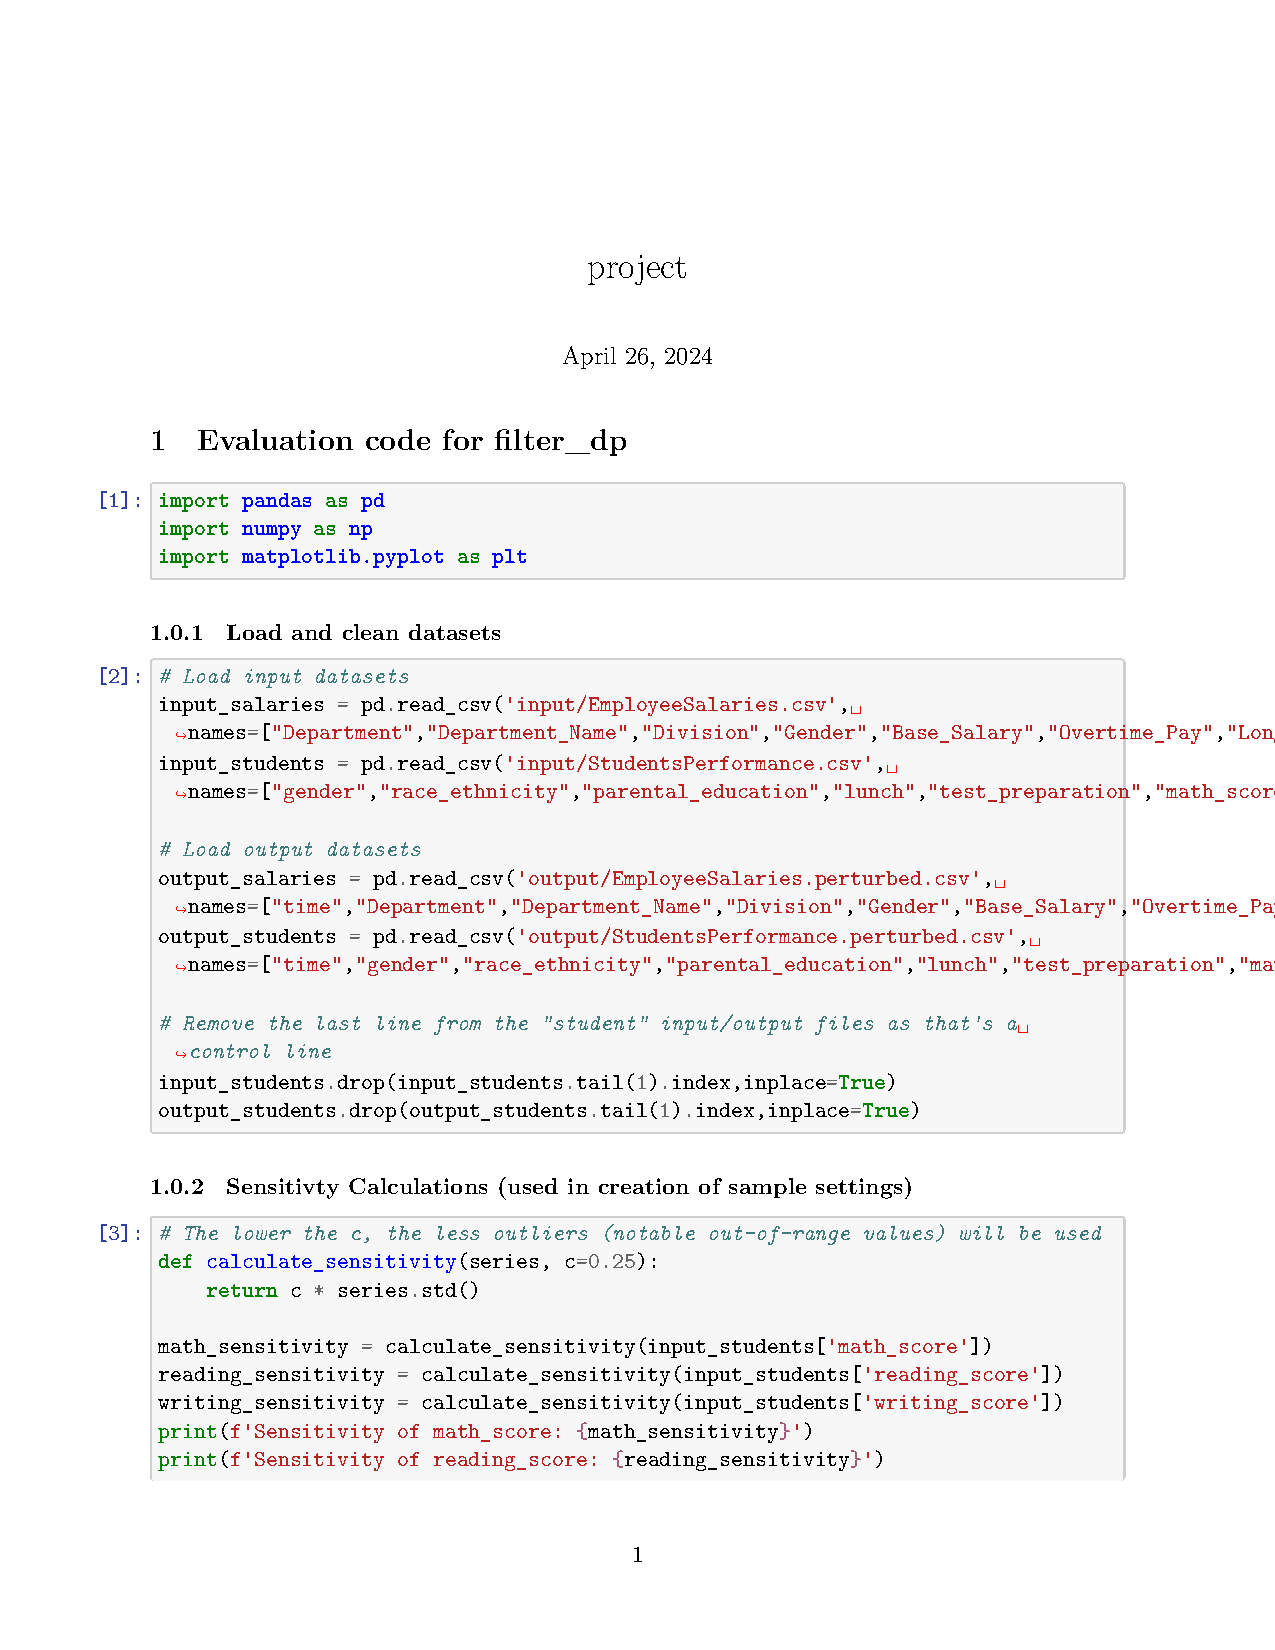
\includepdf[pages=-]{report/media/notebook.pdf}

\bibliography{report/bibliography}

\end{document}
